% This tex file is available under a
% Creative Commons Attribution-Share Alike license (CC BY-SA 2.0).
% http://creativecommons.org/licenses/by-sa/2.0/
% Copyright © 2013 Rodrigo Hausen
\documentclass{beamer}
\usepackage[utf8]{inputenc}
\usepackage{lmodern}
\usepackage[T1]{fontenc}
\usepackage[portuguese,brazil]{babel}
\usepackage{url}
\usepackage{listings}
\usepackage{color}
\usepackage{textcomp}
\usepackage{pdfpages}
\usepackage{fancyvrb}
\usepackage{enumerate}
\usepackage{icomma} % para vírgula decimal / decimal comma
\definecolor{listinggray}{gray}{0.9}
\definecolor{lbcolor}{rgb}{0.9,0.9,0.9}
\lstset{
    backgroundcolor=\color{lbcolor},
    tabsize=4,
    rulecolor=,
    basicstyle=\scriptsize,
    upquote=true,
    aboveskip={1.5\baselineskip},
    columns=fixed,
    showstringspaces=false,
    extendedchars=true,
    breaklines=true,
    prebreak = \raisebox{0ex}[0ex][0ex]{\ensuremath{\hookleftarrow}},
    frame=single,
    showtabs=false,
    showspaces=false,
    showstringspaces=false,
    identifierstyle=\ttfamily,
    keywordstyle=\color[rgb]{0,0,1},
    commentstyle=\color[rgb]{0.133,0.545,0.133},
    stringstyle=\color[rgb]{0.627,0.126,0.941},
}

\definecolor{pinegreen}{RGB}{0,139,114}

\def\A{\texttt{A}}
\def\B{\texttt{B}}
\def\C{\texttt{C}}
\def\D{\texttt{D}}
\def\E{\texttt{E}}
\def\F{\texttt{F}}

\usetheme{Boadilla}
%\usetheme{umbc2}
\usefonttheme{structuresmallcapsserif}
\usecolortheme{seahorse}

\title{Aula 1: Sistemas de Numeração e Bases}
\subtitle{Circuitos Digitais}
\author{Rodrigo Hausen}
\institute{CMCC -- UFABC} 
\date{21 e 23 de janeiro de 2013}

\begin{document}

\begin{frame}
\maketitle

\vspace{-1cm}

\begin{center}
\url{http://compscinet.org/circuitos}
\end{center}

\end{frame}

\begin{frame}
\frametitle{Apresentação}

\begin{itemize}
\item Computador digital:
\pause
\begin{itemize}
\item Aquilo que \textbf{computa}, ou seja, que processa \textbf{informação \pause digital}, ou seja, aquela que é \textbf{quantizada} ou \textbf{discreta} -- ao invés de contínua -- podendo ser representada por números (que possuem \emph{dígitos}).
\end{itemize}
\pause
\item Como um computador digital processa informação? \pause Por meio de \emph{circuitos digitais}
\begin{center}
\includegraphics[height=3cm]{images/HitachiJ100A.jpg}\\[-6pt]
{\color{gray!50!white}\tiny{Fonte: \url{http://en.wikipedia.org/wiki/Digital_electronics}}}
\end{center}
\end{itemize}

\pause

O que são circuitos digitais? \pause Para que me interessa saber o que há em um computador?

\end{frame}


\begin{frame}[fragile] %%% FRAGILE IS VERY IMPORTANT for the listings package!
\frametitle{Um problema...}

Considere o seguinte programa:

\hfill\begin{minipage}{0.95\textwidth}
\lstinputlisting[language=Java,numbers=left]{code/prog1.java}
\end{minipage}

O que será impresso na tela?

\pause

\begin{semiverbatim}
2147483647\pause
-2147483648
\end{semiverbatim}

\end{frame}

\begin{frame}[fragile] %%% FRAGILE IS VERY IMPORTANT!!!
\frametitle{Outro problema...}

\hfill\begin{minipage}{0.95\textwidth}
\begin{lstlisting}[language=Java,numbers=left]
int[][] m = new int[7000][7000];

long start = System.currentTimeMillis();
for (int i=0; i<7000; i++)
    for (int j=0; j<7000; j++)
    {
        m[i][j] = 1;
    }
long stop = System.currentTimeMillis();

System.out.println("Tempo: " + (stop-start) + "ms");\end{lstlisting}
\end{minipage}

\vspace{12pt}

Resultado {\footnotesize (em um Celeron 1.8GHz)}:

\pause

\begin{semiverbatim}
Tempo: 148ms
\end{semiverbatim}

\phantom{Aproximadamente 40 vezes mais lento!?}

\end{frame}

\begin{frame}[fragile] %%% FRAGILE IS VERY IMPORTANT!!!
\frametitle{Outro problema...}

\hfill\begin{minipage}{0.95\textwidth}
\begin{lstlisting}[language=Java,numbers=left]
int[][] m = new int[7000][7000];

long start = System.currentTimeMillis();
for (int i=0; i<7000; i++)
    for (int j=0; j<7000; j++)
    {
        m[j][i] = 1; /* TROQUEI j E i !!! */
    }
long stop = System.currentTimeMillis();

System.out.println("Tempo: " + (stop-start) + "ms");\end{lstlisting}
\end{minipage}

\vspace{12pt}

Resultado {\footnotesize (no mesmo computador)}:

\pause

\begin{semiverbatim}
Tempo: 6117ms
\end{semiverbatim}

Aproximadamente 40 vezes mais lento!?

\end{frame}

\begin{frame}
\frametitle{Desvendando mistérios}

Os comportamentos que vimos nos slides anteriores são devidos à forma como nossos computadores atuais são construídos.

\pause

\vspace{12pt}

\begin{itemize}
\item 1. Quais as suas causas?
\item 2. Podemos prevê-los?
\item 3. Podemos evitá-los?
\end{itemize}

\vspace{12pt}

Para responder essas perguntas, precisamos saber a
\emph{arquitetura do computador} sendo usado. \pause
Para sabermos arquitetura de computadores digitais,
precisamos primeiro entender os seus blocos básicos,
os \emph{circuitos digitais}. \pause
Para conhecermos \emph{circuitos digitais}, precisamos
voltar aos \emph{sistemas de numeração posicionais},
que utilizam \emph{algarismos} (dígitos).
\end{frame}

\begin{frame}
\frametitle{Sistema de numeração}

\begin{itemize}
\item \textbf{Número}: idéia de quantidade
\item \textbf{Numeral}: representação dessa idéia (falada ou escrita)
\end{itemize}

Na prática, usamos a palavra \textbf{número} para nos referirmos também a um \textbf{numeral}.

\pause

\vspace{12pt}

Como representar todos os números naturais possíveis?

\pause

\begin{itemize}
\item Um símbolo para cada número. Ex.: 1, 2, 3, 5, 6, 7, 8, 9, a, b, c, d, e, f, g, h, i, j, k, l, m, n, o, p, q, r, s, t, u, v, w, x, y, z, $\star$, $\dagger$, $\bullet$, \ldots (impossível lembrar todas as representações)
\pause
\item Símbolos diferentes para algumas quantidades, combinações para as demais. Ex.: símbolos no sistema romano são I (um), V (cinco), X (dez), L (cinquenta), C (cem), D (quinhentos), M (mil). Combinações: II (dois), III (três), IV (quatro), MCMLXXXIV (mil novecentos e oitenta e quatro), \ldots
\end{itemize}
\end{frame}

\begin{frame}
\frametitle{Sistema de numeração}

\begin{itemize}
\item \textbf{Algarismos}: conjunto finito de símbolos numéricos que usamos para representar apenas algumas quantidades (não todas).
\pause
\item Todo e qualquer número deve poder ser representado por uma \textbf{combinação} de algarismos 
\pause
\item Exemplo: os algarismos chamados indo-arábicos são $0$, $1$, $2$, $3$, $4$, $5$, $6$, $7$, $8$, $9$.
\pause
\item \textbf{Sistema de numeração}: forma de atribuir uma representação única para cada número.
\pause
\item \textbf{Sistema de numeração posicional}: sistema de numeração onde cada número é representado por uma combinação de algarismos, onde a \textbf{posição} do algarismo altera a quantidade que ele representa.
\end{itemize}

\end{frame}

\begin{frame}
\frametitle{Sistema decimal de numeração posicional}

\begin{itemize}
\item \textbf{Algarismos} ou \textbf{dígitos}: $0$, $1$, $2$, $3$, $4$, $5$, $6$, $7$, $8$, $9$. Por possuir dez algarismos distintos, é chamado \textbf{decimal}.
\pause
\item \textbf{Valor absoluto} de cada algarismo: a quantidade que ele representa. $0$ (zero) = nada, $1$ = um, etc.
\pause
\item Dependendo da \textbf{posição} do algarismo na representação do número, a quantidade que ele representa varia (\textbf{valor posicional} ou \textbf{valor relativo}).
\end{itemize}

\begin{center}
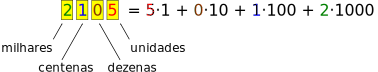
\includegraphics{images/numero2105}
\end{center}

\end{frame}

\begin{frame}
\frametitle{Sistema decimal de numeração posicional}

Em geral, um número inteiro $A$ no sistema decimal é representado por $n$ dígitos
\[
a_{n-1} \; a_{n-2} \ldots a_2 \; a_1 \; a_0
\]
onde cada $a_i$ é um algarismo decimal.\pause Esse numeral representa o número
\[
a_0 \cdot 1 + a_1 \cdot 10 + a_2 \cdot 100 + \ldots a_{n-2} \cdot 10^{n-2} + a_{n-1} \cdot 10^{n-1}
\]
\pause
ou, usando a notação sigma: $\displaystyle \sum_{i = 0}^{n-1} a_i \cdot 10^i$
\end{frame}

\begin{frame}
\frametitle{Números que não são inteiros}

Sejam $A \in \mathbf{Z}$, $B \in \mathbf{N}$ e $Q \in \mathbf{Z}$.

\begin{itemize}
\item Dizemos que $\frac{A}{B} = Q$ se $A = B \cdot Q$ (ou seja, $B$ cabe exatamente $Q$ vezes dentro de $A$). Exemplo: $\frac{6}{2} = 3$ pois $6 = 2 \cdot 3$
\pause
\item Pode acontecer de $B$ não caber um número exato de vezes dentro de $A$. Ou seja, \textbf{resta} uma parte de $A$ que excede $B \cdot Q$. 
\pause
\item Podemos sempre escrever: $A = B \cdot Q + R$, onde $R \in \{0, 1, \ldots, B-1\}$
\pause
\item Chamaremos $Q$ de \textbf{quociente} e $R$ de \textbf{resto} da \textbf{divisão inteira} de $A$ por $B$. Exemplo: na divisão de $7$ por $2$, o quociente é $3$ e o resto é $1$, pois $7 = 2 \cdot 3 + 1$.
\pause
\item Se o resto $R$ da divisão inteira de $A$ por $B$ for diferente de $0$, diremos que a divisão inteira de $A$ por $B$ não é exata.
\pause
\item Um número que pode ser escrito na forma $\frac{A}{B}$, com $A \in \mathbf{Z}$ e $B \in \mathbf{N}$, é chamado racional. O conjunto dos racionais é representado por $\mathbf{Q}$ e inclui os números inteiros e as frações com numerador e denominador inteiros mas cuja a divisão não é exata.
\end{itemize}
\end{frame}

\begin{frame}
\frametitle{Números racionais no sistema decimal}

Todo número racional pode ser representado no sistema decimal da seguinte forma:
\[
a_{n-1} \; a_{n-2} \ldots a_2 \; a_1 \; a_0 , a_{-1} \; a_{-2} \; a_{-3} \; \ldots
\]
onde há um número finito de algarismos à direita da vírgula \textbf{ou} esses algarismos começam a se repetir a partir de uma certa posição.

\pause Esse numeral representa o número $\displaystyle \underbrace{\sum_{i = 0}^{n-1} a_i \cdot 10^i}_{\text{parte inteira}} + \underbrace{\sum_{i = 1}^{\infty} a_{-i} \cdot 10^{-i}}_{\text{parte fracionária}}$

\pause

Ex.: $12,45333\ldots = 1\cdot10 + \pause 2\cdot1 + \pause 4\cdot10^{-1} + \pause 5 \cdot 10^{-2} + \pause 3 \cdot 10^{-3} + \pause 3 \cdot 10^{-4} + \pause 3 \cdot 10^{-5} + \ldots$
\end{frame}

\begin{frame}
\frametitle{Números racionais: truncamento}

\[
a_{n-1} \; a_{n-2} \ldots a_2 \; a_1 \; a_0 , a_{-1} \; a_{-2} \; a_{-3} \; \ldots
\]
Observe que à medida que caminhamos mais para a direita após a vírgula, o valor relativo de cada algarismo torna-se cada vez menor.

\pause

\vspace{12pt}

Podemos tomar uma representação próxima do número, limitando o número de algarismos após a vírgula por uma constante $m$. Esse procedimento de aproximação chama-se \textbf{truncamento} a $m$ dígitos.

\pause

\vspace{12pt}

Ex.: represente a fração $\frac{1007}{495}$ por um numeral truncado a $4$ dígitos decimais e calcule o erro de aproximação.

\pause

\vspace{6pt}

$\frac{1007}{495} = 2,0343434\ldots \pause \approx 2,0343$, usando $4$ dígitos após a vírgula

\pause

\vspace{6pt}

Erro de aproximação:\\$2,0343434\ldots - 2,0343 = 0,000043434\ldots < 10^{-4}$
\end{frame}

\begin{frame}
\frametitle{Números reais: truncamento}

\begin{itemize}
\item \textbf{Se} adotarmos uma representação finita com $m+n$ algarismos para qualquer número real
\[
a_{n-1} \; a_{n-2} \ldots a_2 \; a_1 \; a_0 , a_{-1} \; a_{-2} \; a_{-3} \; \ldots a_{m}
\]
com $n$ algarismos à esquerda da vírgula, e $m$ algarismos à direita,\\\textbf{então} o erro de aproximação de qualquer número será $< 10^{-m}$.

\pause

\item Aumentar $m$ implica a diminuição do erro.

\pause

\item A grande maioria dos números reais que desejamos representar vêm de medidas. Exs: comprimento, temperatura, tempo, etc.

\pause

\item Como toda medida possui um erro $\epsilon$ intrínseco ao processo de medição, podemos escolher $m$ de maneira que o erro de representação seja menor do que o erro de medição. Ou seja, escolha $m$ tal que
\[
10^{-m} < \epsilon \;\; \text{, ou seja, } \;\; m > -\log_{10} \epsilon
\]

\end{itemize}

\end{frame}

\begin{frame}
\frametitle{Bases não decimais}

\begin{itemize}
\item A quantidade de algarismos usados em um sistema de numeração posicional é chamada \textbf{base}.
\pause
\item Ex.: o sistema de numeração decimal é um sistema de base $10$.
\pause
\item A base $10$ tornou-se a mais popular pois possuímos $10$ dedos\\(\emph{digitus} em latim)
\pause
\item Nada impede de construírmos sistemas de numeração posicionais com bases diferentes de $10$ (se tivéssemos apenas $1$ dedo em cada mão, provavelmente a base mais popular seria $2$) 
\pause
\item A base $2$ também é chamada base \textbf{binária}.
\end{itemize}
\end{frame}

\begin{frame}
\frametitle{Bases não decimais}

\begin{itemize}
\item Em um sistema de numeração posicional de base $d$, o número
\[
a_{n-1} \; a_{n-2} \ldots a_2 \; a_1 \; a_0 , a_{-1} \; a_{-2} \; a_{-3} \; \ldots a_{m}
\]
possui valor
\[
    \underbrace{\sum_{i = 0}^{n-1} a_i \cdot d^i}_{\text{parte inteira}} + \underbrace{\sum_{i = 1}^{m} a_{-i} \cdot d^{-i}}_{\text{parte fracionária}}
\]
\pause
\item Para indicar a base em que um número está representado, usaremos a notação
\[
(a_{n-1} \; a_{n-2} \ldots a_2 \; a_1 \; a_0 , a_{-1} \; a_{-2} \; a_{-3} \; \ldots a_{m})_{d}
\]
\end{itemize}

\end{frame}

\begin{frame}
\frametitle{Valor de numerais em base $d$ na base $10$}

Conforme o ditado:\\
``Existem $\uncover<4->{(}10\uncover<4->{)_2}$ tipos de pessoas: \pause aquelas que sabem contar em binário,\\ \pause e as que não sabem.'' \pause

\vspace{12pt}

Exemplos de conversão de base:

\begin{enumerate}
\item $(1{\color{green}1}0{\color{blue}1}00{\color{red}1})_2 = {\color{red}1} \cdot 2^0 + {\color{blue}1} \cdot 2^3 + {\color{green}1} \cdot 2^5 + 1 \cdot 2^6 = 105$
\pause
\item $(110,1001)_2 = 1\cdot2^{-4} + 1\cdot2^{-1} + 1\cdot2^{1} + 1\cdot2^{2} = 6,5625$
\pause
\item $(1{\color{green}1}0{\color{blue}1}00{\color{red}1})_8 = {\color{red}1} \cdot 8^0 + {\color{blue}1} \cdot 8^3 + {\color{green}1} \cdot 8^5 + 1 \cdot 8^6 = 294977$
\pause
\item $(\texttt{B},\texttt{EEF})_{16} = \uncover<8->{11\cdot16^0 +}\uncover<9->{ 14\cdot16^{-1} +}\uncover<10->{ 14\cdot16^{-2} +}\uncover<11->{ 15\cdot16^{-3}}\uncover<12->{ = 11,933}$
\end{enumerate}

Obs.: valor absoluto dos algarismos na base $16$
\begin{tabular}{ccccccccc}
$0$ & \ldots & $9$ & $\texttt{A}$ & $\texttt{B}$ & $\texttt{C}$ & $\texttt{D}$ & $\texttt{E}$ & $\texttt{F}$\\
$0$ & \ldots & $9$ & $10$ & $11$ & $12$ & $13$ & $14$ & $15$
\end{tabular}

\vspace{6pt}

\uncover<13->{A conversão de base $d$ para base $10$ é trivial, pois nossas contas são naturalmente feitas na base decimal!}
\end{frame}

%%%%%%%%%%%%%%%%%%%%%%%%%%%%%%%%%%%%%%%%%%%%

\begin{frame}
\frametitle{Conversão da base $10$ para base $d$}

Vamos começar com os números inteiros.
Exemplo: represente os números $(0)_{10}$, $(1)_{10}$, $(2)_{10}$ e $(3)_{10}$ na base $2$.

\vspace{12pt}
\pause

Muito fáceis: $(0)_{10} = (0)_2$, $(1)_{10} = (1)_2$

\vspace{12pt}
\pause

Não existe nenhum algarismo para representar $(3)_{10}$ na base $2$. Portanto, $(3)_{10}$ deve ser representado como $({\color{blue}a_1} \, {\color{red}a_0})_2$.

\vspace{12pt}
\pause

${\color{red}a_0}$ = unidades, ${\color{blue}a_1}$ = quantidades de $2^1$ em $3$ (ou seja, quantas vezes $2$ cabe em $3$)

\pause

\begin{center}
\begin{tabular}{c|c}
3 & 2 \\
\cline{2-2}
{\color{red}1} & {\color{blue}1}
\end{tabular}

$(3)_{10} = (11)_2$
\end{center}

\end{frame}

%%%%%%%%%%%%%%%%%%%%%%%%%%%%%%%%%%%%%%%%%%%%

\setlength{\unitlength}{15pt}

\newcommand{\R}[1]{{\color{red}#1}}
\newcommand{\ARR}[1]{\begin{picture}(0,0)\put(0,0){\vector(-3,2){#1}}\end{picture}}

\begin{frame}
\frametitle{conversão da base $10$ para base $d$}

Converter $18$ da base $10$ para a base $2$.

\pause

\begin{center}
\begin{tabular}{c c@{}c c@{} c c@{} c c@{} c c l}
\multicolumn{1}{c|}{18} & 2 \\
\cline{2-2}
\multicolumn{1}{c|}{\R0} & 9 \pause & \multicolumn{1}{@{}c|}{} & 2 \\
\cline{4-4}
                         & \R1      & \multicolumn{1}{@{}c|}{} & 4 \pause & \multicolumn{1}{@{}c|}{} & 2 \\
\cline{6-6}
                         &          &                          & \R0      & \multicolumn{1}{@{}c|}{} & 2 \pause & \multicolumn{1}{@{}c|}{} & 2 \\
\cline{8-8}
                         &          &                          &          &                          & \R0      & \multicolumn{1}{@{}c|}{} & 1 \pause & \multicolumn{1}{@{}c|}{} & 2 \\
\cline{10-10}
                         &          &                          &          &                          &          &                          & \R1      & \multicolumn{1}{@{}c|}{} & 0 & \pause quociente 0 = terminou! \pause \\[-6pt]
                         &          &                          &          &                          &          &                          & \ARR{5} \\ 
                         &          &                          &          &                          &          &                          &         & \multicolumn{3}{l}{leia os restos neste sentido}
\end{tabular}
\end{center}

\pause

$(18)_{10} = (10010)_2$

\end{frame}

%%%%%%%%%%%%%%%%%%%%%%%%%%%%%%%%%%%%%%%%%%%%

\begin{frame}
\frametitle{conversão da base $10$ para base $d$}

Converter $731$ da base $10$ para a base $2$.

\pause

\begin{center}
\begin{tabular}{c c@{}c c@{} c c@{} c c@{} c c@{} c c@{} c c@{} c c@{} c c@{} c c l}
\multicolumn{1}{c|}{731} & 2 \\
\cline{2-2}
\multicolumn{1}{c|}{\R1} & 365 \pause & \multicolumn{1}{@{}c|}{} & 2 \\
\cline{4-4}
                         & \R1        & \multicolumn{1}{@{}c|}{} & 182 \pause & \multicolumn{1}{@{}c|}{} & 2 \\
\cline{6-6}
                         &            &                          & \R0        & \multicolumn{1}{@{}c|}{} & 91 \pause & \multicolumn{1}{@{}c|}{} & 2 \\
\cline{8-8}
                         &            &                          &            &                          & \R1       & \multicolumn{1}{@{}c|}{} & 45 \pause & \multicolumn{1}{@{}c|}{} & 2 \\
\cline{10-10}
                         &            &                          &            &                          &           &                          & \R1       & \multicolumn{1}{@{}c|}{} & 22 \pause & \multicolumn{1}{@{}c|}{} & 2 \\
\cline{12-12}
                         &            &                          &            &                          &           &                          &           &                          & \R0       & \multicolumn{1}{@{}c|}{} & 11 \pause & \multicolumn{1}{@{}c|}{} & 2 \\
\cline{14-14}
                         &            &                          &            &                          &           &                          &           &                          &           &                          & \R1       & \multicolumn{1}{@{}c|}{} & 5 \pause & \multicolumn{1}{@{}c|}{} & 2 \\
\cline{16-16}
                         &            &                          &            &                          &           &                          &           &                          &           &                          &           &                          & \R1      & \multicolumn{1}{@{}c|}{} & 2 \pause & \multicolumn{1}{@{}c|}{} & 2 \\
\cline{18-18}
                         &            &                          &            &                          &           &                          &           &                          &           &                          &           &                          &          &                          & \R0      & \multicolumn{1}{@{}c|}{} & 1 \pause & \multicolumn{1}{@{}c|}{} & 2 \\
\cline{20-20}
                         &            &                          &            &                          &           &                          &           &                          &           &                          &           &                          &          &                          &          &                          & \R1      & \multicolumn{1}{@{}c|}{} & 0 \\ \pause
\\
                         &            &                          &            &                          &           &                          &           &                          &           &                          &           &                          &          &                          &          &                          & \ARR{14}
\end{tabular}
\end{center}

\vspace{-36pt}

\pause

$(731)_{10} = (1011011011)_2$

\end{frame}

%%%%%%%%%%%%%%%%%%%%%%%%%%%%%%%%%%%%%%%%%%%%

\begin{frame}
\frametitle{conversão da base $10$ para base $d$}

Converter $731$ da base $10$ para a base $16$.

\pause

\begin{center}
\begin{tabular}{c c@{}c c@{}c c l}
\multicolumn{1}{c|}{731} & 16 \\
\cline{2-2}
\multicolumn{1}{c|}{\R{11}} & 45\pause & \multicolumn{1}{@{}c|}{} & 16 \\
\cline{4-4}
                         & \R{13}   & \multicolumn{1}{@{}c|}{} & 2  \pause & \multicolumn{1}{@{}c|}{} & 16 \\
\cline{6-6}
                         &          &                          & \R2       & \multicolumn{1}{@{}c|}{} &  0 \\ \pause
                         &          &                          & \ARR{4}
\end{tabular}
\end{center}

\pause

Observe que $(11)_{10} = (B)_{16}$ e que $(13)_{10} = (D)_{16}$, logo\\[12pt]

$(731)_{10} = (2DB)_{16}$

\end{frame}
%%%%%%%%%%%%%%%%%%%%%%%%%%%%%%%%%%%%%%%%%%%%

\begin{frame}
\frametitle{conversão da base $10$ para base $d$}

      $(18)_{10} = (10010)_2$ \\
$(731)_{10} = (1011011011)_2$ \\[12pt]

Observação 1:
\begin{itemize}
\item se um número é \textbf{par}, na base $2$ o seu último algarismo é sempre $0$
\item se um número é \textbf{ímpar}, na base $2$ o seu último algarismo é sempre $1$
\end{itemize}

\vspace{12pt}

Observação 2: é muito fácil converter da base $2$ para $16$ e vice-versa!

\vspace{16pt}

\only<2>{$(731)_{10} = (10{\color{blue}1101}{\color{red}1011})_2$}%
\uncover<3->{$(731)_{10} = (\underbrace{10}_{2_{16}}\underbrace{\color{blue}1101}_{{\color{blue}D}_{16}}\underbrace{\color{red}1011}_{{\color{red}B}_{16}})_2$}
\uncover<4->{$= (2{\color{blue}D}{\color{red}B})_{16}$}\\[12pt]

\only<5>{$(\hspace{7pt}5\hspace{15.7pt}0\hspace{13pt}F\hspace{13.5pt}1\hspace{15.5pt}A\hspace{8pt})_{16}$}%
\uncover<6->{$(\underbrace{5}_{(0101}\underbrace{0}_{0000}%
\underbrace{F}_{1111}\underbrace{1}_{0001}\underbrace{A}_{1010)_2})_{16}}$%

\end{frame}

%%%%%%%%%%%%%%%%%%%%%%%%%%%%%%%%%%%%%%%%%%%%

\begin{frame}
\frametitle{Para casa}

\begin{itemize}
\item Acessar o site \url{http://compscinet.org/circuitos} e ler as informações sobre o curso com cuidado
\pause
\item Obter o livro:\\
Thomas Floyd. Sistemas Digitais: Fundamentos e Aplicações, 9ed. Editora Bookman, 2007.
\pause
\item Leitura recomendada: Floyd, seções 2-1 a 2-6 (menos a parte de números em ponto flutuante), 2-7, 2-8.
\item Exercícios recomendados: autoteste 1 a 16, problemas de 1 a 40 (exceto 27 e 28)
\end{itemize}

\end{frame}

\end{document}
